% Roll Number 3, Abilash Sajeev

\textbf{\textcolor{LightMagenta}{Write down the major differences between K-means clustering and hierarchical clustering. (May 2019) \hfill 4 marks}} \\[5pt]
\textcolor{purple}{\underline{\textbf{K-Means Clustering}}}\\
K-Means clustering intends to partition n objects into k clusters in which each object belongs to the cluster with the nearest mean. This method produces exactly k different clusters of greatest possible distinction. The best number of clusters k leading to the greatest separation (distance) is not known as a priori and must be computed from the data. The main objective of the K-Means algorithm is to minimize the sum of distances between the points and their respective cluster centroid. \\ 
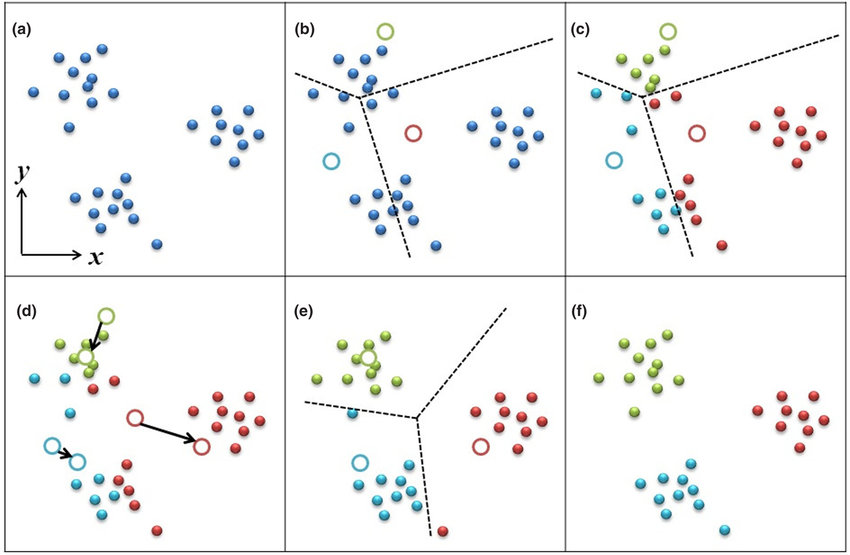
\includegraphics[scale=0.45]{Images/A33_img1.png} 
\\ \\
\textcolor{purple}{\underline{\textbf{Hierarchical Clustering}}}\\
Hierarchical clustering, also known as hierarchical cluster analysis, is an unsupervised clustering algorithm which involves creating clusters that have predominant ordering from top to bottom. The algorithm groups similar objects into groups called clusters. The endpoint is a set of clusters, where each cluster is distinct from each other cluster, and the objects within each cluster are broadly similar to each other. \\
This clustering technique is divided into two types: 
\begin{itemize}
    \item {Agglomerative Hierarchical clustering Technique} 
    \item {Divisive Hierarchical clustering Technique} 
\end{itemize}

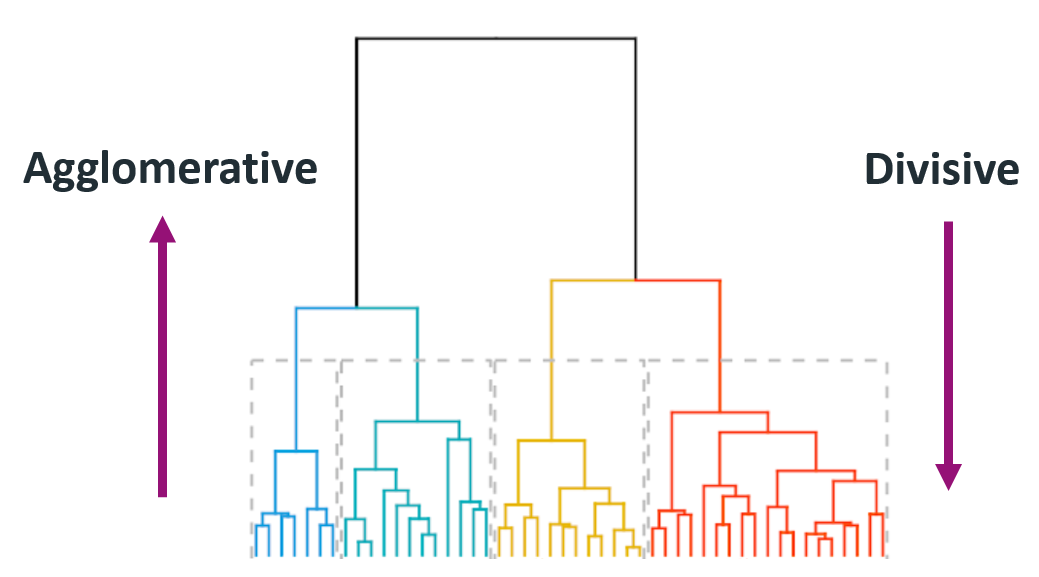
\includegraphics[scale=0.40]{Images/A33_img2.png} 

\textcolor{purple}{\underline{\textbf{Difference between K-Means and Hierarchical clustering}}}
\begin{itemize}
    \item Hierarchical clustering can’t handle big data well but K-Means clustering can. This is because the time complexity of K-Means is linear i.e. O(n) while that of hierarchical clustering is quadratic i.e. O(${n^2}$). 
    \item In K-Means clustering, since we start with random choice of clusters, the results produced by running the algorithm multiple times might differ. While results are reproducible in Hierarchical clustering. 
    \item K-Means clustering requires prior knowledge of K i.e. no. of clusters you want to divide your data into. But you can stop at whatever number of clusters you find appropriate in hierarchical clustering by interpreting the dendrogram.
    \item K-means clustering produces a single partitioning. Hierarchical clustering can give different partitioning depending on the level of resolution we are looking at. 
    \item The result of K-means is unstructured, but that of hierarchal is more interpretable and informative.
    \item K-means clustering a simply a division of the set of data objects into non-overlapping subsets(clusters) such that each data object is in exactly one subset. A hierarchical clustering is a set of nested clusters that are arranged as a tree.
    \item K-Means clustering is found to work well when the structure of the clusters is hyper spherical (like circle in 2D, sphere in 3D). Hierarchical clustering doesn’t work well when the shape of the clusters is hyper spherical.
    
\end{itemize} \\